\documentclass[a4paper,openright,12pt]{report}

\usepackage[spanish]{babel}
\usepackage{longtable}
\usepackage{xcolor}
\usepackage{enumitem}
\usepackage{amsmath}
\usepackage{mathtools}
\usepackage{fixltx2e}
\usepackage{hyperref}
\usepackage[T1]{fontenc}
\usepackage[utf8]{inputenc}
\usepackage{graphicx}
\usepackage{apacite}
\usepackage[autostyle]{csquotes}
\usepackage{framed}
\usepackage{titlesec}
\usepackage{floatrow}
\usepackage[list=true]{subcaption}
\usepackage{url}

\setcounter{secnumdepth}{5}

\hypersetup{
    colorlinks,
    citecolor=blue,
    filecolor=blue,
    linkcolor=black,
    urlcolor=blue
}

\hyphenation{re-no-ván-do-se}
\hyphenation{e-le-men-to}
\urlstyle{same}
\setlength{\parskip}{1em}

% Support older LaTeX versions.
\DeclareUnicodeCharacter{2060}{}

\begin{document}
\begin{titlepage}
	\centering

	{\sffamily\large\bfseries PONTIFICIA UNIVERSIDAD CATÓLICA DEL PERÚ \par}
	\vspace{0.2cm}
	{\sffamily\large\bfseries INGENIERÍA INFORMÁTICA\par}
	\vfill

	
\includegraphics[width=6cm]{../images/logo-pucp.png}\par\vspace{1cm}
	\vspace{1.5cm}

	{\sffamily\large\bfseries Implementación de un plug-in para GStreamer para
	el seguimiento de rostros aplicado a Cheese\par}
	\vspace{2cm}

	{\sffamily\small Tesis para optar por el título de Ingeniero Informático que
		presenta el bachiller: }

	{\sffamily\Large\bf	César Fabián Orcccón Chipana \par}
	{\sffamily 20105515 \par}
	\vfill
	{\sffamily Asesor: Dr.~Ivan \textsc{Sipiran} \par}

	\vfill

% Bottom of the page
	{\sffamily\large \today\par}
\end{titlepage}



\tableofcontents
\chapter{Generalidades}
\section{Problemática}


Por más de 130 años las personas han usado cámaras para documentar sus vidas
\cite{snap2017prospectus}.
Cuando las primeras cámaras fueron inventadas, era difícil y costoso tomarse una
fotografía \cite{snap2017prospectus}. Un filtro fotográfico es un accesorio para las
cámaras fotográficas que se inserta en la parte frontal de esta para conseguir
cierto efecto deseado. La historia de los filtros fotográficos también es muy
antigua, y se remonta al siglo XIX. En 1878, Frederick Wratten, un innovador e
investigador del campo de la fotografía introdujo un proceso conocido como
“noodling” que permitía crear placas fotográficas más sensitivos que las
existentes en esa época \cite{hannavy2013encyclopedia}⁠. En 1906, él junto con
su hijo y el doctor C. E. Kenneth
Mees fundaron una compañía llamada Wainwright Ltd., en la cual Mees ayudó a
Wratten a desarrollar las primeras placas pancromáticas y los primeros filtros
de luz, los cuales se harían conocidos como Wratten filters
\cite{hannavy2013encyclopedia}⁠. Kodak compraría
más tarde Wainwright Ltd. en el 1912 \cite{hannavy2013encyclopedia}⁠. Desde
entonces, los filtros fotográficos han ganado popularidad, y renovándose hasta
la actualidad.\\

En las dos últimas décadas, la aparición de la fotografía digital ha dejado
atrás a las cámaras de película \cite{CIPAfilmCameraStats}. En la actualidad,
es común contar si no con una cámara digital, entonces al menos con una cámara
web integrada al computador personal portátil o al telefóno inteligente. El
término “filtro” (el cual de aquí y en
adelante será entendido como “filtro digital”) también se ha mudado al contexto
digital y se ha introducido en el hablar del común de muchas personas. Las
razones por las cuales las personas aplican filtros a sus fotografías son
varias. Algunos aplican filtros para mejorar la estética regulando el brillo,
contraste y focalización \cite{bakhshi2015we}. Otros desean aplicar efectos
antiguos, por ejemplo algunos colocan las fotografías en blanco y negro para
concentrar la atención en cierta textura de la toma y evitar que el espectador
se distraiga en los colores, otros simplemente desean darle un aspecto de
antigüedad \cite{bakhshi2015we}. Otras personas simplemente desean cambiar los
colores \cite{bakhshi2015we}. Finalmente, algunos otros simplemente
desean darle un aspecto único y divertido a las fotografías
\cite{bakhshi2015we}. El único propósito de estos últimos es el agregar
características divertidas (a través de filtros) que no pudieron ser capturadas
originalmente por la cámara \cite{bakhshi2015we}.\\

Hoy en día, diversas empresas se han apalancado del fácil acceso a la cámara web
por parte de los usuarios de teléfonos inteligentes destacando entre ellas
empresas como Skype Technologies S.A.R.L (Skype), Oath Inc. (Flickr),
Facebook Inc. (Facebook e Instagram) y Snap Inc. (Snapchat) han permitido la
edición de imágenes aplicando filtros de manera sencilla para sus usuarios. Por
ejemplo, la aplicación para móviles Snapchat se ha hecho muy popular por no solo
aplicar filtros que permiten regular los colores de la foto o video en tiempo
real, sino que permite detectar objetos capturados por la cámara del dispositivo
y seleccionar entre una diversa variedad de lentes que permite sobreponer
animaciones interactivas sobre la toma \cite{snap2017prospectus}⁠. Este tipo de
filtros se han popularizado especialmente entre “millennials”. Por ejemplo, para
Snapchat, los jóvenes de entre 18 y 24 años representan un 36\% de sus usuarios
activos por día en Estados Unidos \cite{snap2017prospectus}⁠. De hecho, muchos
jóvenes adultos sostienen que este tipo de filtros resuelve problemas de
comunicación dado en ciertas redes sociales debido a que la sobreposición de
imágenes y texto puede clarificar el mensaje que ellos desean expresar en sus
fotografías \cite{vaterlaus2016snapchat}. El deseo por agregar stickers sobre
las fotografías, no se limita a occidente. De hecho, esta práctica ha sido y es
muy común en Japón desde la década de los noventas. En el año 1995, Altus, una
empresa japonesa, desarrolló un fotomatón (un quiosco para tomarse fotos,
generalmente insertando una moneda) que permitía agregar stickers sobre las
fotografías \cite{edwards2004photographs}. Atlus patentó una máquina con el
nombre de Purikura, término que se volvería más adelante en un término del uso
cotidiano de las personas en Japón principalmente los adolescentes
\cite{edwards2004photographs}. Recientemente, estas máquinas también se han
renovado incluyendo filtros digitales para el agregado de “stickers” sobre las
fotografías \cite{TheOrigi29}.\\

En las computadoras de escritorio, podemos dividir la situación actual de las
aplicaciones de webcam por el Sistema Operativo en los cuales están soportadas.
Por un lado, en macOS, la aplicación para capturar fotos y videos con la cámara
web por defecto es Photo Booth, la cual permite aplicar filtros en tiempo real,
así como detectar a una persona para reemplazar el fondo por un video
preestablecido o foto colocada manualmente por el usuario \cite{photoBooth}. Fun
Booth es una aplicación para macOS. desarrollada por Spoonjuice LLC, la cual
permite detectar un rostro humano frente a la cámara para colocar stickers sobre
este \cite{funBooth}. Por otro lado, Windows 10 incluye una aplicación para la toma de fotos y grabación de
video, pero esta no dispone de filtros tan sofisticados como los de Photo Booth.
Sin embargo, existen aplicaciones de terceros con varias funcionalidades.
CyberLink YouCam, de CyberLink Corp. permite no solo detectar el rostro del
individuo capturado y sobreponer filtros sobre esto, sino que detecta las
emociones de las personas \cite{YouCam7A82}⁠. ManyCam que entre diversas
funcionalidades que ofrece, permite además aplicar filtros para colocar máscaras
y animaciones que rastrean el rostro de la persona ubicada frente a la webcam
\cite{Webcamso75}. Para sistemas operativos basados en GNU/Linux, existen
programas que permiten ajustar los colores de las capturas con la cámara web,
pero la aplicación, al parecer, más popular y a la vez con filtros más
sofisticados es Cheese, proyecto de la GNOME Foundation \cite{AppsChee13}.⁠\\

Cheese, a diferencia del resto de programas mencionados con licencia privativa,
es un software libre \cite{cheeseLicense}⁠. El software libre a diferencia del software privativo,
según la Free Software Foundation, es el software que respeta la libertad de sus
usuarios y comunidad permitiéndoles tener el derecho de ejecutar, copiar,
distribuir, estudiar, modificar y mejorar el programa \cite{whatIsFreeSoftware}⁠.
Cheese está licenciado bajo la licencia GNU General Public License versión 2
(GPLv2) \cite{cheeseLicense}⁠.
El hecho de que este tenga una licencia libre es fundamental para el desarrollo
de este proyecto de fin de carrera, pues permite a otros estudiar su código
fuente, mejorarlo y modificarlo. Este software, además, ha sido financiado por
Alphabet Inc. en varias ocasiones. De hecho, este fue inicialmente desarrollado
en el 2007 por Daniel G. Siegel como parte de un proyecto del Google Summer of
Code (GSoC), programa ideado por Larry Page y Sergey Brin, fundadores de Google,
para difundir el software libre y de código abierto remunerando a estudiantes
por desarrollar en este tipo de proyectos \cite{gsoc1}.\\


La necesidad por agregar soporte para sobreposición de imágenes sobre el rostro
de las capturas de Cheese fue expresado en el 2010 ⁠\cite{Bug6279256} y, además
ya hubo intentos de agregar esta funcionalidad. En el GNOME Outreach Program for
Women (programa para mujeres similar al GSoC pero financiado por la GNOME
Foundation, ahora llamado Outreachy) del 2010, la participante Laura Elisa Lucas
Alday, trabajó en desarrollar un filtro (elemento) para GStreamer llamado
gstfaceoverlay, el cual permitía la adición de imágenes en formato svg sobre un
rostro detectado en una imagen \cite{faceoverlay}\cite{gopw1}. El
filtro fue aceptado por los desarrolladores GStreamer, y posteriormente agregado
a GNOME Video Effects, librería que contiene una lista de filtros o combinación
de filtros de GStreamer en archivos de texto y que son usados por Cheese para
aplicar los filtros. Sin embargo, este filtro fue posteriormente retirado de
GNOME Video Effects puesto que algunos archivos svg hacían lento (el “framerate”
caía) a Cheese \cite{Bug6641489}.\\


En setiembre 2012, GStreamer 1.0 fue lanzado, y desde esa fecha, gstfaceoverlay
no fue portado a la nueva versión de GStreamer. Esto llevó a que el filtro fuera
borrado de la librería el 21 de diciembre del 2016. Ante esto, en el 2016, se
propuso un parche en el "bug tracker" de GNOME para portar el filtro a las
series GStreamer 1.x, el cual sería aceptado en GStreamer en el año 2017
\cite{Bug7640127}. Una vez portado, se probó su funcionamiento en Cheese
\cite{CFOCHfunnyStickersCheese} y se observó que además de solo soportar la
sobreposición de imágenes con formato SVG, este filtro no puede detectar el
rostro de más de una persona. Ello condujo a proponer otro parche que solucione
este problema \cite{Bug7691771}. Sin embargo, esta solución si bien al parecer
es correcta en un contexto aislado, arrastra un problema en su base. El problema
fundamental en este filtro es que no ha debido implementarse sobre la base del
filtro gstfacedetect. De hecho, usar gstfacedetect como base es un error si se
desea usar el plugin en Cheese para dar soporte a múltiples rostros con
múltiples imágenes, pues este aplica la detección facial para cada cuadro (o
\textit{“frame”} en inglés), pero sin respetar un orden alguno, es decir que una persona
etiquetada en el primer cuadro con la imagen A podría ser etiquetada en el
segundo marco con la imagen B, y en el tercero otra vez con A o tal vez con C.
Lo esperado sería que si se sobrepuso la imagen A sobre el rostro de una
persona, esta imagen A se mantenga sobrepuesta en los siguientes cuadros.\\

Para conseguir que Cheese soporte filtros de sobreposición de imágenes sobre los
rostros de personas en tiempo real no es suficiente escribir un nuevo filtro
para GStreamer. Tampoco es suficiente, luego de escribir el filtro, agregar la
configuración del “pipeline” de GStreamer a GNOME Video Effects de tal modo que
Cheese pueda leerlo. Cheese debería implementar una interfaz gráfica en la cual
el usuario pueda seleccionar e importar imágenes que desea usar, de este modo no
se evita el uso de efectos estáticos predeterminados. Es preciso resaltar que
realizar tales cambios a Cheese no es fácil para nuevos colaboradores del
proyecto. Cheese no se ha actualizado recientemente, y una de las razones puede
ser que existe pocas personas que sepan programar en Vala, un lenguaje de
programación orientado a objetos con un compilador que traduce el
código a C para compilarlo compilado con gcc \cite{valaOverview}. Además Cheese usa Clutter,
librería de GNOME basada en OpenGL, para mostrar la salida de la captura y los
efectos aplicados en la pantalla. Ambos no disponen de mucha documentación
disponible pública, y por lo general, uno debe guiarse en base a otros programas
que han sido escritos usando tanto Clutter como Vala. Por otro lado, entre los
filtros a usar para el rastreamiento de imágenes, algunos como face4d no tienen
licencias compatibles con GPLv2, para lo cual no solo es necesario escribir
software libre, sino que el código debe ser compatible con esta licencia.\\

En conclusión, se puede observar que los usuarios de software para la cámara web
tienen varias razones para preferir usar filtros. El problema es más acentuado para
usuarios de software libre. Los programas de escritorio con licencias libres o
de código abierto para capturar imagen y video están quedándose atrasados
tecnológicamente. Sin embargo, el problema no solo está en este tipo de software,
sino que pareciera que las aplicaciones para macOS también están en la misma
situación. Recientemente, la aparición de Snapchat ha creado una tendencia entre
millennials de 18 a 24 años a tener una preferencia por filtros que sobreponen
imágenes que siguen sus rostros capturados por la cámara web a otros medios
de comunicación convencionales. Siendo Cheese un software libre, lo cual
representa una ventaja social sobre el software privativo, es posible estudiarlo
y mejorarlo (sin mencionar otras libertades), además, se considera como la mejor
opción para desarrollar este proyecto pues tiene mejores características en
comparación de otros proyectos con licencias libres. Agregar la funcionalidad de
aplicar filtros que sobrepongan imágenes sobre los rostros de las personas
capturados por una webcam en tiempo real no solo es beneficio para los jóvenes
millennials, sino también para la GNOME Foundation y podría aumentar la
competitividad entre aplicaciones de escritorio de captura de video y entre
entornos de escritorio para sistemas basados en UNIX (incluyendo macOS).

\section{Objetivos}
\subsection{Objetivo general}
Implementar e integrar en Cheese un plugin (un conjunto de elementos) para
GStreamer que mediante el uso de algoritmos para detección y seguimiento de
múltiples rostros (o una adaptación de estos) permita sobreponer imágenes sobre
los rostros detectados en videos (particularmente, por la cámara web).

\subsection{Objetivos específicos}
\subsubsection{OE0: Objetivo Específico 0}
Desarrollar un algoritmo que implemente un filtro para GStreamer para
la detección y rastreamiento de múltiples rostros con soporte para oclusión
entre rostros.
\subsubsection{OE1: Objetivo Específico 1}
Escribir el código fuente de un filtro para GStreamer que basado en el filtro
implementado en \textit{OE0} permita detectar el "landmark" de cada rostro.
\subsubsection{OE2: Objetivo Específico 2}
Escribir el código fuente de un filtro para GStreamer que basado en el filtro
implementado en \textit{OE1} permita la sobreposición de imágenes sobre puntos
predeterminados en los rostros detectados.
\subsubsection{OE3: Objetivo Específico 3}
Diseñar una interfaz gráfica para Cheese que permita al usuario de Cheese
aplicar el filtro implementado en \textit{OE2}.

\subsection{Resultados esperados}
\subsubsection{REOE0: Resultados esperados para el Objetivo Específico 0}
Un filtro que sea al menos tan preciso como alguno de los algoritmos de rastreo
de múltiples rostros estudiados en este proyecto de fin de carrera y
además que otorgue suficiente fluidez lo cual un manejo adecuado del retardo en
GStreamer. Este filtro deberá además definir una estructura extendible, la cual
contiene los datos de las coordenadas de los rostros rastreados y se envía como
un mensaje al bus.
\subsubsection{REOE1: Resultados esperados para el Objetivo Específico 1}
Un filtro que tomando las coordenadas del filtro implementado para \textit{OE0}
permita detectar el landmark de los rostros detectados además de extender el
mensaje recibido en el bus por el filtro del OE0 para también enviar las
coordenadas de los puntos del landmark como mensaje en el bus.
\subsubsection{REOE2: Resultados esperados para el Objetivo Específico 2}
Un filtro que tomando como referencia las coordenadas de diversos puntos de cada
rostro detectado ofrezca un conjunto de propiedades para colocar imágenes en
lugares predefinidos del rostro como filtrum (parte entre la boca y nariz),
boca, ojos, nariz, orejas y cara.
\subsubsection{REOE3: Resultados esperados para el Objetivo Específico 3}
Una interfaz gráfica con un conjunto de imágenes clasificadas por categoría. De
estas imágenes el usuario puede seleccionar una o más de estas imágenes las
cuales serán sobrepuestas en los rostros detectados aplicando el filtro del
\textit{OE2}.

\subsection{Herramientas, métodos y procedimientos}

\subsubsection{En relación al Objetivo Específico 0 (OE0)}
\paragraph{Metodologías y algoritmos para el seguimiento de rostros}\mbox{} \\

Según Zaheer Shaik y Vijayan Asari, los métodos de seguimiento de personas
pueden ser clasificados en cuatro categorías según la forma, las características,
el modelo o color de piel de la cara \cite{shaik2007robust}. Estos se detallan
a continuación:

\begin{enumerate}
    \item Seguimiento basado en la forma: en este método se debe usar un modelo
    que represente la locación de una cara. Se toma la elipse como el modelo más
    simple que mejor se ajusta a la forma de una cara \cite{eleftheriadis1995automatic}. Este método de
    seguimiento no es influenciado por el color de fondo ni por los cambios en
    la iluminación \cite{shaik2007robust}. Sin embargo, este falla si la cara rastreada es ocluida ya
    sea por otro objeto u otra persona \cite{shaik2007robust}.
    \item Seguimiento basado en características:  en este método, las
    características de los rostros son extraídas usando el filtro de Gabor el
    cual es usado como característica para el seguimiento de rostros \cite{shaik2007robust}. Sin
    embargo, este método no es sensible a los cambios en iluminación y la pose
    de la cara \cite{shaik2007robust}. Hacer que este método soporte esta característica tiene un alto
    costo computacional por lo que no es adecuado para streaming.
    \item Seguimiento basado en el modelo: este usa un modelo en 3D del rostro,
    el cual es proyectado en los cuadros detectados por la cámara \cite{shaik2007robust}. Sin embargo,
    estos pueden tener dificultad cuando hay cambios de iluminación o si la cara
    es ocluida \cite{smolyanskiy2014real}. Si bien esta metodología suele ser precisa tiene el problema de
    tener un alto costo computacional por lo que no es adecuado para streaming.
    \item Seguimiendo en base a los colores: este método usa el modelo de color
    de piel \cite{shaik2007robust}. Sin embargo, aunque falla cuando el rostro es ocluido, es adecuado
    para streaming.
\end{enumerate}

A continuación se describirán algunos métodos y algoritmos usados para el
seguimiento de rostros basados en el método en base al color de la piel.

\subparagraph{A Real-time Model for Multiple Human Face Tracking from Low-resolution Surveillance Videos}\mbox{} \\

Es un método propuesto por Rajib Sarkara, Sambit Baksh y Pankaj K Sa. Ha sido
probado en 1000 imágenes elegidas al azar de la base de datos de rostros
frontales de personas de Europa, Asia y África \cite{sarkar2012real}.
Su exactitud es del 96.2\% \cite{sarkar2012real}.
Además, con imágenes con resolución reducida a través de interpolación este
algoritmo tiene un comportamiento más eficiente \cite{sarkar2012real}.
A continuación se describen los pasos que sigue:
\begin{enumerate}[label=(\alph*)]
    \item Detectar y segementar las regiones de piel en una imagen
        \cite{sarkar2012real}. Para ello se usa el siguiente algoritmo:
    \begin{framed}
    \textbf{Entrada}: Una imagen $I$ en el modelo de color \textit{RGB} de
    dimensión.\\
    \textbf{Salida}: Una imagen binaria $S$ indicando si un pixel es piel o no.\\
    \textbf{Pasos}:\\
        \begin{enumerate}[label=\arabic*.]
            \item Convertir la imagen $I$ de \textit{RGB} a
                \textit{YC\textsubscript{b}C\textsubscript{r}}.
            \item Calcular la luma promedio de una imagen $I$ calculado como
                \[
                    {}_{I}Y_{prom} = {\sum_{i=1}^{m}\sum_{i=1}^{n} {}_{I}Y_{i,j}} 
                \]
            \item Normalizar ${}_{I}Y_{i,j}$ a ${[0,255]}$
            \item Encontrar el mapa de contornos usando el detector de bordes de
                Canny para la imagen de entrada \textit{RGB}.
            \item Encontrar la imagen compensada de brillo ${}_{I}C'$ obtenido
                de la siguiente manera:\\
                \textit{Cada pixel}
                    ${}_{I}C'_{i,j} = \{{}_{I}R'_{i,j}, {}_{I}G'_{i,j}, {}_{I}B'_{i,j}\}$
                \textit{donde:}\\
                \[
                    {}_{I}R'_{i,j} = ({}_{I}R'_{i,j})^\tau
                    {}_{I}G'_{i,j} = ({}_{I}G'_{i,j})^\tau
                    {}_{I}B'_{i,j} = ({}_{I}B'_{i,j})^\tau
                \]
                \textit{para:}
                \begin{equation}
                    \tau=
                    \begin{cases}
                        1.5, & \text{if }\ {}_{I}Y_{prom}<64\\
                        0.7, & \text{if }\ {}_{I}Y_{prom}>190\\
                        1
                    \end{cases}
                \end{equation}
            \item El mapa de colores de piel para ${}_{I}C'_{i,j}$ es calculado
                como:
                \begin{equation}
                    S_{i,j}=
                    \begin{cases}
                        0, & \text{if $\frac{R + 1}{G + 1}>1.08$ y $\frac{R + 1}{B + 1}>1.08$ y $G>30$ y $G<140$}\\
                        1
                    \end{cases}
                \end{equation}
                donde $S_{i,j}=0$ indica una región de piel y $S_{i,j}=0$ lo contrario.
        \end{enumerate}
        \raggedleft\cite{sarkar2012real}
    \end{framed}

    \item Verificar si cada componente de la piel corresponde (o no) a un
        rostro verificando la existencia de la boca y ojos \cite{sarkar2012real}.
    \item Colocar un cuadro en cierta orientación sobre la región de piel
        detectada dependiendo de la forma de la cara \cite{sarkar2012real}.
\end{enumerate}

\subparagraph{A Robust Method for Multiple Face Tracking Using Kalman Filter}\mbox{} \\

Es un método propuesto por Zaheer Shaik y Vijayan Asari para el seguimiento de
múltiples rostros. Este resuelve el problema de oclusiones parciales y totales 
tomando como referencia el modelo de la ropa de las personas \cite{shaik2007robust}. Además también
supera los problemas de iluminación y cambios en las poses, velocidades y
trayectorias de los rostros \cite{shaik2007robust}. A continuación se describe la metodología empleada 
en más detalle.\\

Cada rastreador de rostro se inicia usando el algoritmo de detección de rostros
de Viola-Jones el cual se provee en \textit{OpenCV}, además se inician las
plantillas (\textit{templates} en inglés) de los rostros \cite{shaik2007robust}. Las caras detectadas
se limitan por un ROI rectangular \cite{shaik2007robust}. En este instante, también se inicia el modelo
de ropa que se usará para cada persona al cual corresponde a una función de
distribución de densidad no paramétrica \cite{shaik2007robust}. Como la distribución, de antemano, no
es conocida se usa una estimación de densidad (\textit{kernel}) tomando como
\textit{kernel} la función de Epanechnikov \cite{shaik2007robust}. De esta manera, la función de
distribución de la ropa para una región $q_{u}$ se calcula de la siguiente
manera:
\[
    q_{u} = C{\sum_{i,j} k(\lVert x_{ij} \rVert^2)\delta[b(x_{ij}) - u]}
\]
donde $\delta$ es la función de Kronecker, $k$ el \textit{kernel} de
Epanechnikov y $b$ es la función que asocia un pixel $x$ en la posición $ij$
a un índice $b(x_{ij})$ en un espacio de colores cuantificada (es decir en un
espacio de colores reducido) \cite{shaik2007robust}.\\

Además se usa el filtro de Kalman, el cual es un filtro usado para la estimación
de ciertas variables en el futuro con aplicaciones en predicción de análisis
financieros, navegación y control de vehículos, procesamiento de señales,
econometría y seguimiento de gráficos interactivos por computadora
\cite{bishop2001introduction}. Para ello, se usan cinco variables: $x_{t}$ 
y $y_{t}$ que corresponden a la posición de la esquina superior izquierda de los
rectángulos que bordean los rostros detectados, $y'_{t}$ y $y'_{t}$ que
representan las velocidades, y por último, el ancho del rectángulo $W_{t}$
\cite{shaik2007robust}. La altura no se considera, pero se asume igual a $1.25$
veces el ancho \cite{shaik2007robust}. A continuación se muestra el modelo de
estados usado (siendo las variables con sufijo ${t + 1}$ las coordenadas
predichas y $w_{t}$ el ruido gausiano):
\[
    \begin{bmatrix}
        x_{t+1}\\
        y_{t+1}\\
        x'_{t+1}\\
        y'_{t+1}\\
        W_{t+1}
    \end{bmatrix}
    =
    \begin{bmatrix}
        1   &   0   &   \Delta{t}   &   0           &   0\\
        0   &   1   &   0           &   \Delta{t}   &   0\\
        0   &   0   &   1           &   0           &   0\\
        0   &   0   &   0           &   1           &   0\\
        0   &   0   &   0           &   0           &   1\\
    \end{bmatrix}
    \begin{bmatrix}
        x_{t}\\
        y_{t}\\
        x'_{t}\\
        y'_{t}\\
        W_{t}
    \end{bmatrix}
    +
    w_{t}
\]
Estas variables predichas se usan para localizar un rostro en el frame
"actual" \cite{shaik2007robust}. Usando una técnica de coincidencia de plantillas o (\textit{template
matching} en inglés), se calcula la distancia entre la plantilla de una cara del
cuadro anterior y de la región con los valores predichos \cite{shaik2007robust}. Si el cuadro anterior
es menor a un \textit{threshold} de 0.9, se asume \textbf{oclusión parcial} \cite{shaik2007robust}.
Además basándose en las coordenadas para el cuadro "actual" halladas por el
filtro de Kalman, se recalcula el modelo de distribución de la ropa para el
cuadro actual ($p_{u}$) \cite{shaik2007robust}. Luego se debe medir la similitud entre las
distribuciones $q_{u}$ y $p_{u}$ \cite{shaik2007robust}. Para ello se usa la métrica estadística
conocida como la distancia de Bhattacharyya la cual es dada por
$\rho = \sum_{u}\sqrt{(p_{u}.q_{u})}$ \cite{shaik2007robust}. Si $\rho$ es menor que un
\textit{threshold} de 0.5, se asume que los modelos no son similares y deben de
ser actualizados \cite{shaik2007robust}.\\
Para actualizar el \textit{template} de rostro se debe redetectar los rostros en
el frame actual \cite{shaik2007robust}. Para ello, se usa una técnica basada en los colores \cite{shaik2007robust}. Tomando el
espacio de color cuantificado (reducido), se busca clasificar los pixeles como
"tipo piel" o "no tipo piel" \cite{shaik2007robust}. Para ello se usa el espacio de color
\textit{YC\textsubscript{b}C\textsubscript{r}}, en el cual la luma \textit{Y} es
separada: ello hace este algoritmo robusto a cambios en la iluminación. Luego,
estos pixeles son clasificados como piel según un threshold en los rangos de
$[100,135]$ y $[135,170]$ para C\textsubscript{b} y C\textsubscript{r},
respectivamente \cite{shaik2007robust}. Una vez identifacadas las regiones de piel, se agrupan los
pixeles de una región para la detección del rostro \cite{shaik2007robust}. La primera etapa consiste en
erosionar la imagen de la región de la cara usando una elipse, para luego
erosinarlas con el fin de llenar los huecos dejados entre los rostros. El
resultado es una máscara binaria de \textit{blobs} de las regiones de los
rostros \cite{shaik2007robust}.\\

Para detectar la región al rededor de cada \textit{blob} se usa un algoritmo
de detección de bordes el cual es implementado por \textit{OpenCV} \cite{shaik2007robust}. Luego, a los
contornos detectados se les aplica un parámetro estadístico llamado el
coeficiente de suavidad para cada "blob" \cite{shaik2007robust}. Si el coeficiente para un
\textit{blob} es menor a $0.5$, este se descarta \cite{shaik2007robust}.\\

En los \textit{blobs} restantes, se aplica un "factor de forma", el cual
relaciona el área entre el perímetro \cite{shaik2007robust}. Este se compara al "factor de forma"
mínimo calculado para los primeros rectángulos que limitaban los rostros
detectados cuando se usó Viola-Jones \cite{shaik2007robust}. El fin de esto es eliminar más
\textit{blobs} \cite{shaik2007robust}. Luego para los \textit{blobs} que sobraron, se dibujan los
rectángulos tomando solo en consideración el ancho del \textit{blob} \cite{shaik2007robust}.\\

Una vez detectados los rostros, si el número de caras detectados es menor al
número de caras rastreadas, se asume oclusión total \cite{shaik2007robust}. Luego, si existe más
rostros de los clasificados como haber sido objetivo de rastreo en un cuadro
anterior, se dice que un nuevo rostros existe (por ejemplo, entra una nueva
persona a la zona de grabación) \cite{shaik2007robust}. Luego, la ecuación de medición del filtro de Kalman, se actualiza según:
\[
    \begin{bmatrix}
        mx_{t+1}\\
        my_{t+1}\\
        mW_{t+1}
    \end{bmatrix}
    =
    \begin{bmatrix}
        1   &   0   &   \Delta{t}   &   0           &   0\\
        0   &   1   &   0           &   \Delta{t}   &   0\\
        0   &   0   &   0           &   0           &   1\\
    \end{bmatrix}
    \begin{bmatrix}
        x_{t - \Delta{t}}\\
        y_{t - \Delta{t}}\\
        x'_{t - \Delta{t}}\\
        y'_{t - \Delta{t}}\\
        W_{t - \Delta{t}}
    \end{bmatrix}
    +
    v_{t}
\]
donde $mx_{t+1}$, $my_{t+1}$ y $mW_{t+1}$ corresponden a variables de medición,
y $v_{t}$ es el ruido de medición, representado por ruido gausiano \cite{shaik2007robust}. Así las
variables son actualizadas en el cuadro actual tomando el pasado (el cuadro
anterior) \cite{shaik2007robust}. Esto permite al algorimo seguir múltiples rostros de personas en el
caso de oclusión, variación de luz y el cambio de la pose \cite{shaik2007robust}.


\paragraph{Herramientas empleadas}\mbox{} \\
\begin{enumerate}
    \item OpenCV, ya que implementa algunos algoritmos y técnicas
        útiles para el seguimiento y detección de rostros:
    \begin{enumerate}
        \item Conversión a espacios de color, usado para trabajar las imágenes
            RGB en distintos espacios de color entre estos \textit{GRAY} y
            \textit{YC\textsubscript{b}C\textsubscript{r}}.
        \item Filtro de Kalman, usado para la predicción de variables en base
            a un modelo y variables de medición.
        \item \textit{Canny Edge Detector}, el cual permite identificar los
            contornos presentes en una imagen.
        \item Erosión y dilatación de imágenes.
    \end{enumerate}
    \item \textit{GStreamer}, ya que es el framework sobre el cual se
        implementará el filtro.
    \item \textit{gstfacedetect}, filtro para \textit{GStreamer} que usa OpenCV
        para la detección de rostros y envía señales al \textit{bus} con las
        coordenadas localizadas.
    \item C++, ya que OpenCV y GStreamer lo soportan.
    \item gst-launch-1.0 para probar manualmente la salida del streaming.
    \item gst-validate para validar que el filtro implementado no produzca
        frames cuando recibe una señal EOS (end-of-stream) o que reciba frames
        mientras esté en el estado \textit{PAUSED}
\end{enumerate}

\subsubsection{En relación al Objetivo Específico 1 (OE1)}
\begin{enumerate}
    \item Dlib, ya que permite detectar el landmark de un rostro.
    \item \textit{GStreamer}, \textit{C++, gst-launch-1.0} y \textit{gst-validate}
        por las mismas razones mencionadas en el caso anterior.
\end{enumerate}

\subsubsection{En relación al Objetivo Específico 2 (OE2)}
\begin{enumerate}
    \item \textit{gdkpixbufoverlay}, un filtro para \textit{GStreamer} que permite la
        sobreposición de imágenes sobre los cuadros recibidos por este filtro.
    \item \textit{GStreamer}, \textit{C++, gst-launch-1.0} y \textit{gst-validate}
        por las mismas razones mencionadas en el caso anterior.
\end{enumerate}

\subsubsection{En relación al Objetivo Específico 3 (OE3)}
\begin{enumerate}
    \item \textit{Gtk+}, librería para diseñar interfaces gráficas para GNOME,
        la cual es usada por \textit{Cheese} y se usará para diseñar la
        interfaz gráfica para seleccionar las imágenes a sobreponer sobre
        los rostros.
    \item \textit{Galde}, una interfaz gráfica en GTK+ para construir interfaces
        gráficas en GTK+.
    \item \textit{Vala}, lenguaje en el cual se desarrolla \textit{Cheese}.
    \item \textit{GStreamer}, integrando los filtros implementados con
        \textit{Cheese}.
    \item \textit{GLib Test Suite}, para ejecutar pruebas sobre el nuevo código
        agregado a \textit{Cheese}.
\end{enumerate}



\section{Alcance, limitaciones y riesgos}

\subsubsection{Alcance}
    Este proyecto se concentrará en funcionar en las computadoras por lo menos
    tres años antiguas. Es decir, la detección, seguimiento y sobreposición de imágenes en
    Cheese debería dar la sensación de fluidez a usuarios de estas computadoras.
    Además, este proyecto debe funcionar sobre \textit{Wayland} ya que es el
    protocolo más usado recientemente por las distribuciones de GNU/Linux
    reemplazando a \textit{X.Org}.

\subsubsection{Limitaciones}

\begin{enumerate}
    \item Si bien lo esperado es que el resultado de este proyecto de fin de
        carrera sea incluido lo más pronto posible en \textit{Cheese} esto puede
        que no suceda en el corto plazo debido a complejidades las cuales deben
        ser tomadas en cuenta pero alargarían la complejidad del proyecto. Por
        lo que el código resultante se garantiza que será nada más que una rama
        (\textit{git branch}) de \textit{Cheese}. Los motivos por lo cual la
        inclusión de este proyecto en la rama \textit{master} de \textit{Cheese}
        puede demorar se detalla en las siguientes líneas.
    \item \textit{Cheese} es uno de los programas de software libres más
        populares para la captura de fotos y video por cámara web. Cabe
        resaltar que este viene incluido también en Ubuntu una de las
        distribuciones de GNU/Linux más populares. Ubuntu y otras distribuciones
        no incluyen ni OpenCV ni dlib por defecto en su distribución, y es poco
        probable que lo haga solo para soportar \textit{Cheese}.
    \item Una de las razones por las cuales las distribuciones de GNU/Linux no
        estarían dispuestas a aceptar los nuevos cambios en \textit{Cheese}
        puede ser por un tema de rendimiento o para evitar ocupar más espacio en
        disco de lo que ocupan usualmente. Las distribuciones en GNU/Linux más
        populares por lo general, están pensadas en dar soporte y estabilidad
        en computadoras muy antiguas. Este proyecto de fin de carrera no tiene
        la intención de dar soporte a computadoras muy antiguas ya que exigiría
        más tiempo de trabajo para mejorar el rendimiento de los algoritmos.
    \item Debido a estos problemas mencionados, lo más indicado sería
        desarrollar esta nueva funcionalidad como un programa extra a
        \textit{Cheese}, de tal modo que por ejemplo un usuario de Ubuntu pueda
        simplemente instalar la funcionalidad de sobreposición de imágenes sobre
        los rostros con un comando, por ejemplo,
        \textit{sudo apt-get install cheese-face-stickers}. O incluso un
        proyecto más complejo podría ser el desarollp de un gestor de
        \textit{plugins} para \textit{Cheese} usando \textit{Libpeas} y brindar
        este proyecto como un \textit{plug-in}. Sin
        embargo, esto no hace más que extender el trabajo y tiempo, por lo que
        lo expuesto no se hará, y como se mencionó el trabajo será limitado
        a una rama de \textit{Cheese}. Si el trabajo es mezclado en
        \textit{master} sin implementar lo sugerido será simplemente una
        coincidencia.
    \item Otra solución sería distribuir \textit{Cheese} en Flatpak. Eso tampoco
        se espera hacer ya que \textit{Cheese} no está actualmente integrado con
        \textit{Flatpak} aunque es una solución altamente recomendable.
\end{enumerate}

\subsubsection{Riesgos}
Un proyecto de fin de carrera puede estar asociado a diversos riesgos. Los
riesgos listados en la tabla de abajo no solo implican situaciones del mismo
proyecto, sino también riesgos externos los cuales pueden afectar negativamente
el desarrollo de este proyecto.


\begin{center}
  \begin{longtable}{| p{.4\textwidth} | p{.15\textwidth} | p{.4\textwidth} |}
  \hline

  \textbf{Riesgo identificado} &
  \textbf{Impacto} &
  \textbf{Medidas para mitigar el riesgo}
  \\ \hline

  Una mala planificación del proyecto puede no solo retrasar el cumplimiento de
  los respectivos entregables sino en el peor de los casos, el incumplimiento
  del mismo. &
  Alto &
  Organizar los tiempos adecuadamente con el fin de evitar retrasos.
  \\ \hline

  La brecha de seguridad, principalmente a través de un ataque cibernético por
  \textit{hackers} puede poner en riesgo cuentas donde se tiene publicados los
  avances del proyecto de fin de carrera. Estas amenazas puede incluir acceso
  no autorizado a cuentas como \textit{github}, \textit{Google Drive} y
  correo electrónico del autor del proyecto.&
  Medio&
  Mantener los avances del proyecto en más de una cuenta, y evitar limitarse
  a una sola cuenta.
  \\ \hline

  La aparición de \textit{blocker bugs} en actualizaciones de dependencias
  pueden impactar negativamente en el cumplimiento del cronograma previsto y
  además afectar la compatibilidad del software presentado con las últimas
  versiones en dependencias. &
  Bajo &
  Los \textit{blocker bugs} suelen ser temporales, por tanto, si en el
  transcurso del proyecto apareciera alguno, se debería reportar el \textit{bug}
  en caso de no estar reportado y simplemente esperar hasta que aparezca una
  actualización. Mientras tanto se deberá trabajar sobre una versión anterior
  de la dependencia.
  \\ \hline

  La repentina enfermedad del autor de este proyecto podría retrasar la
  entrega de entregables, lo cual a su vez conllevaría retrasos en revisiones o
  en la no revisión del proyecto por parte del asesor asignado y profesores.&
  Medio &
  El autor del proyecto deberá tomar medidas de prevención para su salud como
  una dieta saludable y tratar dormir 8 horas pese a que al alto volumen de
  trabajo, al parecer no anticipado, por algunos cursos universitarios los cuales
  podrían afectar negativamente la salud tanto mental como física tanto en el
  corto como en el largo plazo \cite[p.~10-11]{estresAcademico}.
  \\ \hline

  Actualizaciones y cambios radicales en las librerías como \textit{GStreamer},
  \textit{OpenCV} y \textit{dlib} que cambien la forma de trabajo puede retrasar
  el avance del desarrollo del software debido a que implicará un esfuerzo extra
  el aprender la nueva forma de uso de estos programas. &
  Bajo &
  Estar al pendiente de páginas, blogs, foros y listas de correos de las
  respectivas librerías con el fin de estar al tanto de las últimas
  actualizaciones con el fin de evitar de que el software use funciones
  obsoletas.
  \\ \hline

  La indisponibilidad del asesor asignado puede afectar negativamente el
  proceso de revisión, y por tanto la calidad, del proyecto. &
  Medio &
  Se deberá solicitar la asignación de un asesor con el conocimiento en el área
  relacionada.
  \\ \hline

  \end{longtable}
\end{center}


\section{Viabilidad}
\subsection{Viabilidad técnica}
\subsection{Viabilidad temporal}
\subsection{Viabilidad económica}
\chapter{Marco Conceptual}
\section{Objetivos del marco conceptual}
A continuación se explicará algunos conceptos que se consideran básicos para
poder comprender los siguientes capítulos \cite{shaik2007robust}. En primer lugar, se explica qué es
el software libre ya que a veces es un concepto que suele ser confundido. Luego,
se introduce a GStreamer, librería en la cual Cheese se basa. Finalmente, se
muestra una visión en conjunto del flujo de datos multimedia en Cheese, así como
las librerías que se usarán para implementar los algoritmos de seguimiento de
rostros.

\section{Software libre}
El software libre es el software que respeta la libertad de sus usuarios y
comunidad. Según la Free Software Foundation, para que un programa
informático sea calificado de software libre, su licencia debe otorgar las
siguientes cuatro libertades:
\begin{framed}
\begin{quote}
\begin{itemize}
\item La libertad de ejecutar el programa como se desea, con cualquier propósito
(libertad 0).
\item La libertad de estudiar cómo funciona el programa, y cambiarlo para que
haga lo que usted quiera (libertad 1). El acceso al código fuente es una condición
necesaria para ello.
\item La libertad de redistribuir copias para ayudar a su prójimo (libertad 2).
\item La libertad de distribuir copias de sus versiones modificadas a terceros
(libertad 3). Esto le permite ofrecer a toda la comunidad la oportunidad de
beneficiarse de las modificaciones. El acceso al código fuente es una condición
necesaria para ello.
\end{itemize}
\raggedleft\cite{cuatroLibertades}
\end{quote}
\end{framed}
Si estas cuatro libertades no se cumplieran, el software se consideraría no
libre. Como se puede observar además, el término “precio” no se ha mencionado.
Por lo que el software libre no es un tema de precios, sino como se mencionó
inicialmente, de libertad, lo cual está relacionado directamente con un tema
ético \cite{cuatroLibertades}. Sin embargo, se aclara esto ya que muchos suelen
confundirlo con “freeware”.
\section{Software no libre o software privativo}
El software no libre también llamado software privativo es todo software que no
cumple alguna de las cuatro libertades del software libre, y por tanto no es
software libre \cite{gnuCategories}.
\section{GNOME}
Es un entorno de escritorio para distribuciones de GNU/Linux y BSD. Está
desarrollado por The GNOME Project, parte del proyecto GNU. GNOME es software
libre y está formado por una amplia variedad de proyectos más pequeños los
cuales están licenciados en su mayoría bajo las licencias GPL y LGPL. GNOME
está financiado por algunas empresas grandes como Google Inc. y Red Hat Inc
\cite{GNOMEFoundation}. Entre estos proyectos se encuentran librerías
importantes como un conjunto de librerías para la creación de programas para
el usuario final y programas para el usuario final como editores de texto como
un navegador de archivos, un emulador de terminal, navegadores web, clientes
IRC, programas gráficos para el control de versiones en Git, reproductores de
audio y video, visores de imágenes entre una lista de más de cien proyectos
\cite{GNOMEProjects}. GNOME es uno de lo escritorios libres más populares y
está traducido en más de 40 idiomas \cite{GNOMETranslationTeams}.

\section{GStreamer}
Es un proyecto de GNOME. GStreamer es una librería de código abierto y
multiplataforma escrita en C con bindings en varios otros lenguages de
programación y basada en GObject. GStreamer implementa un modelo de
“pipelines” que enlaza una serie de elementos, por ejemplo, demultiplexores,
decodificadores, multiplexores, filtros y codificadores \cite{GStreamerFeatures}.
Ello permite que cada elemento cumpla una tarea específica. GStreamer permite
la creación de aplicaciones multimedia y streaming. Para ejemplificar,
considerar el caso de la reproducción reproducción de un archivo con formato
ogg, se puede pasar el elemento a un elemento llamado gstfilesrc, donde este lee
el archivo por buffers y pasa un buffer a un demuxer que separa el audio del
video. Los buffers de audio van a un decodificador de Vorbis (códec de audio),
mientras que los buffers de video son pasados a un decodificador de Theora
(códec de vídeo).
Cada buffer de audio es pasado a un elemento que se encargará de pasar los datos
recibidos, por ejemplo, a PulseAudio. Cada buffer de video, por su parte, podría
ser enviado a Wayland. PulseAudio se encargaría de trasladar esos datos al
driver de audio para emitir la salida por el parlante y Wayland se encargaría
de mostrar el video en pantalla.
\subsection{Elemento (GstElement)}
Un elemento (GstElement) Es una abstracción sobre la cual se basan la mayoría de
objetos de GStreamer para construir un pipeline, el cual es una cadena de
objetos GstElement enlazados. Un GstElement puede tener una entrada y una o más
salidas. En un demultiplexor gstoggdemux por ejemplo, la entrada serían buffers
del archivo en formato ogg, y las salidas serían por un lado, el audio, y por
el otro lado el vídeo.\\
Existe tres tipos de elementos muy usados:\\
\subsubsection{Sources}
Son productores de datos, puede ser por ejemplo \textit{gstvideotestsrc} que
produce datos para videos de prueba; otro ejemplo, podría ser
\textit{gstfilesrc} que carga datos de un archivo. Los source elements solo
tienen un source pad.

\begin{figure}[h]
  \centering
    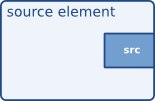
\includegraphics{../images/pwg-src-element.png}\par
  \caption{Representación de un \textit{source}}
  \floatfoot{Fuente: \cite[p.~5]{boulton2017gstreamer}}
\end{figure}

\subsubsection{Sinks}
Representan consumidores de datos. Por ejemplo, \textit{glimagesink} recibe
frames en un buffers y los renderiza usando OpenGL mostrando el resultado en una
ventana. \textit{waylandsink}, \textit{xvimagesink}, \textit{cluttersink}
cumplen roles similares pero usan internamente Wayland, X y Clutter
respectivamente. Un "sink element" solo tiene un sink pad.

\begin{figure}[h]
  \centering
    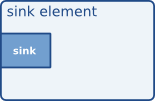
\includegraphics{../images/pwg-sink-element.png}\par
  \caption{Representación de un \textit{sink}}
  \floatfoot{Fuente: \cite[p.~5]{boulton2017gstreamer}}
\end{figure}

\subsubsection{Filtros}
Un filtro recibe ciertos datos, los procesa, y envía los datos modificados por
una o más salidas. Un ejemplo de filtro es agingtv que agrega un efecto de
televisión antigua. Otro ejemplo es \textit{glfiltercube} que usa OpenGL para
crear un cubo cuyas caras están texturizadas con los frames que este filtro
recibe. Un filtro tiene un source pad y un sink pad.

\begin{figure}[h]
  \centering
    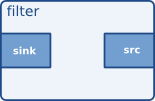
\includegraphics{../images/pwg-filter-element.png}\par
  \caption{Representación de un filtro}
  \floatfoot{Fuente: \cite[p.~5]{boulton2017gstreamer}}
\end{figure}

\subsubsection{Bin}
Un \textit{bin} es un tipo de elemento que contiene más elementos. La cantidad
de \textit{source pads} que posee y la cantidad de sink pads (ambos llamados
\textit{ghost pads} cuando se trata de un \textit{bin}) que posee puede ser
variable, y por lo general, depende de los elementos que están en sus extremos.

\begin{figure}[h]
  \centering
    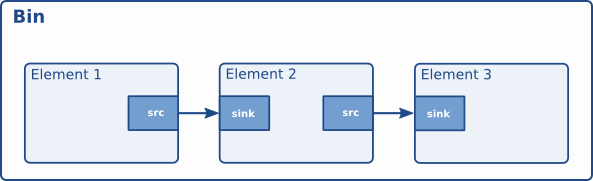
\includegraphics[width=\textwidth]{../images/ad-bin.png}\par
  \caption{Representación de un \textit{bin}}
  \floatfoot{Fuente: \cite{taymans2016gstreamer}}
\end{figure}


\subsubsection{Pipeline}
Es, por lo general, el bin de máximo nivel en una aplicación. Un
\textit{pipeline} controla el reloj (\textit{GstClock}) global del cual dispone
GStreamer, además dispone de un bus el cual controla, por lo que la aplicación
no tiene la necesidad de crear un bus. Un pipeline puede recibir consultas de
la aplicación como por ejemplo para hacer seeking o para obtener duración del
video reproducido con el pipeline.

\begin{figure}[h]
  \centering
    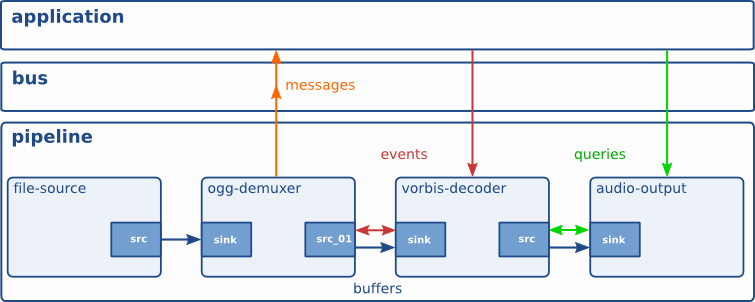
\includegraphics[width=\textwidth]{../images/ad-pipeline.png}\par
  \caption{Representación de un \textit{pipeline}}
  \floatfoot{Fuente: \cite{taymans2016gstreamer}}
\end{figure}

\subsection{Bus (GstBus)}
GStreamer es una librería multihilo. Cada GStreamer el bus es el encargado de
recibir mensajes del pipeline y enviarlos a la aplicación. La aplicación puede
capturar estos mensajes usando un \textit{callback} (similar a un
\textit{signal handler}). Por ejemplo, \textit{facedetect} usa \textit{OpenCV}
para detectar los rostros, y el tamaño y coordenadas de los rostros detectados
son enviadas al bus. De esta manera, una aplicación u otro elemento como
\textit{gstfaceoverlay} puede leer los mensajes en el bus y decidir qué hacer
con la información recibida, en este caso sobreponer imágenes.
\subsection{Plugin (GstPlugin)}
GStreamer es extendible a través de plugins. Un plugin puede contener uno o un
conjunto de elementos. Un plugin no es un elemento. En GStreamer, entre los
sets de plugins más populares se encuentran:
\begin{itemize}
\item \textbf{gst-plugins-base} es un set de plugins con los elementos esenciales para
la creación de elementos más complejos.
\item \textbf{gst-plugins-good} es un set de plugins soportado activamente por
la comunidad de GStreamer. Está licenciado bajo LGPL.
\item \textbf{gst-plugins-ugly} también licenciado bajo la licencia LGPL
(versión 2.1), es un set de plugins que puede carecer de revisiones, un
mantenedor activo, documentación, pruebas unitarias o cuyos desarrolladores
pueden tener dudas respecto a ciertas patentes.
\item \textbf{gst-plugins-bad} es un set de plugins que puede tener problemas
de distribución.
\end{itemize}
\section{Clutter}
Es una librería que usa OpenGL para crear interfaces gráficas ocultando la
complejidad de este mismo. Coloca a la disposición del desarrollador
herramientas para agregar texto, animaciones, imágenes los cuales, por ejemplo,
pueden ser arbitrariamente colocados o rotados \cite{clutterOverview}. Clutter
se integra tanto con Gtk como con Gstreamer.
\section{Vala}
Es un lenguaje de programación orientado a objetos desarrollado para adaptarse
mejor a las librerías de GNOME. El compilador de Vala es valac, el cual compila
código en Vala, generando archivos del lenguaje C, los cuales son compilados con
\textit{gcc}. La orientación a objetos está dada debido a que internamente usa
GObject, librería de GNOME que simula la programación orientada a objetos en C.
El hecho de que compilar programas escritos en Vala genere código fuente en C,
la necesidad de escribir bindings. Sintácticamente, es idéntico a C\#
\cite{valaOverview}.
\section{GNOME Video Effects}
Es una colección de filtros de GStreamer \cite{GNOMEVideoEffects} guardados en
archivos de texto con un título, una pequeña descripción y la descripción del
\textit{pipeline}.
\section{Cheese}
Es un proyecto de GNOME nacido en el 2007 como parte de un proyecto de Google
Summer of Code. Escrito inicialmente por el entonces estudiante Daniel G. Siegel
y mantenido actualmente por David King. Cheese es un programa para capturar
fotos y videos con la cámara web con la opción de aplicar filtros. Está
licenciado bajo la licencia GPLv2, y escrito principalmente en el lenguaje de
programación Vala, aunque con partes escritas en C \cite{cheeseReferenceManual}
\cite{cheeseApp}.\\

\begin{figure}
\begin{subfigure}{0.4\textwidth}
  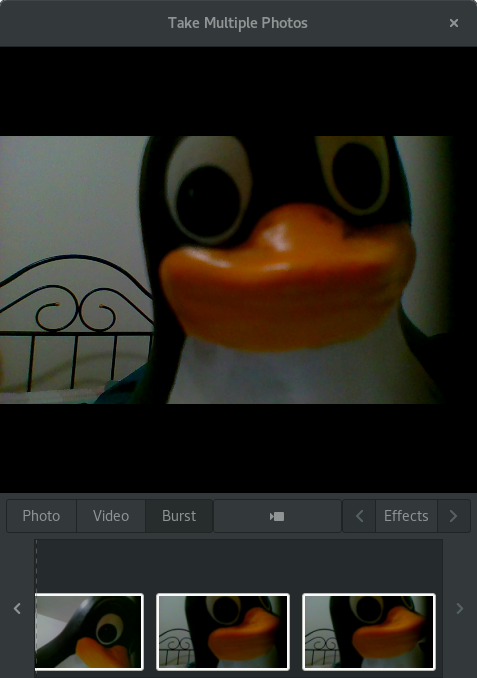
\includegraphics[width=\textwidth]{../images/cheese-viewport.png}
  \caption{Ventana principal de Cheese}
\end{subfigure}
\hfill\vrule\hfill
\begin{subfigure}{0.4\textwidth}
  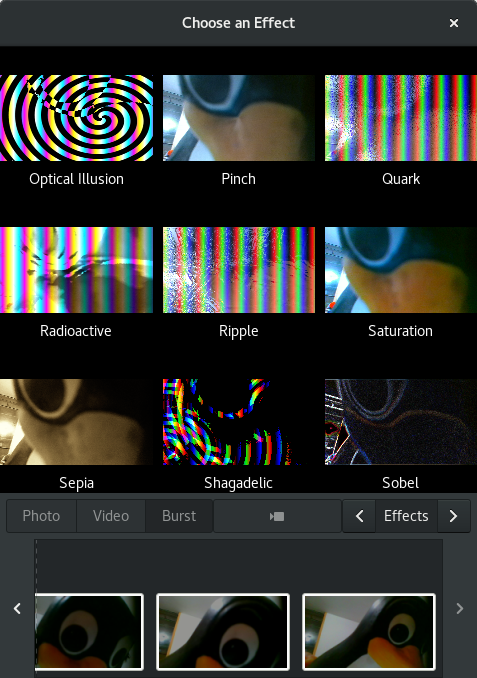
\includegraphics[width=\textwidth]{../images/cheese-effects-grid.png}
  \caption{Ventana de efectos de Cheese}
\end{subfigure}
\caption[Hello]{Cheese}
\floatfoot{Fuente: autoría propia}
\end{figure}

Cheese lee los filtros o efectos de GNOME Video Effects y los usa para
mostrarlos en su interfaz gráfica. Tanto la captura de videos (o fotos) como la
aplicación de filtros en Cheese está dada internamente por GStreamer, un
framework que permite el desarrollo de aplicaciones multimedia. Cheese crea
internamente una pipeline bastante compleja, de la cual se muestra una
simplificación en el diagrama de la \textit{figura 2.7}. El diagrama ignora
elementos como \textit{capsfilters}, \textit{bins} y algunos otros filtros y
elementos.

\begin{figure}
  \centering
    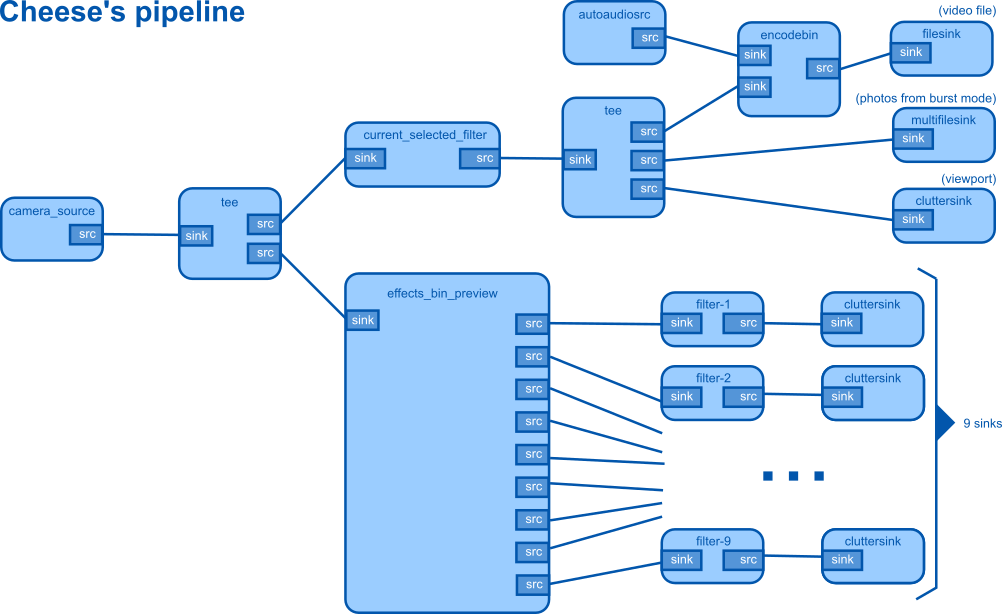
\includegraphics[angle=90,width=0.8\textwidth]{../images/cheese-pipeline.png}\par
  \caption{Simplificación del \textit{pipeline} de Cheese. Imagen inspirada a
  				 partir de la generación de un diagrama en Graphviz con GStreamer en
  				 modo DEBUG}
  \floatfoot{Fuente: Autoría propia}
\end{figure}

\section{OpenCV}
Es una librería para visión artificial en tiempo real. Es software de código
abierto siendo licenciada bajo la licencia BSD. Fue inicialmente desarrollado
por Intel Inc \cite{openCVAbout}. Está escrita en C y C++ con bindings para
otros lenguajes de programación como Python y Java. Entre los distintos
algoritmos que implementa OpenCV se encuentra la detección de objetos usando
el algoritmo propuesto por Paul Viola y Michael Jones en “Rapid Object Detection
using a Boosted Cascade of Simple Features” y el algoritmo para la estimación de
 variables llamado filtro de Kalman. \cite{openCVAbout}.
\section{dlib}
Es una librería que implementa una amplia cantidad de algoritmos en aprendizaje
de máquina. Es software de código abierto licenciado bajo la
licencia Boost License y escrita en C++ \cite{dlib}\cite{dlibLicense}. Entre
los distintos algoritmos que implementa se encuentra el propuesto por Navneet
Dalal y Bill Triggs en “Histograms of Oriented Gradients for Human Detection”
\cite{dlibHOG} y la detección del “landmark” del rostro con el algoritmo
propuesto por Vahid Kazemi y Josephine Sullivan en “One Millisecond
Face Alignment with an Ensemble of Regression Trees” \cite{dlib1ms}.

\chapter{Estado del Arte}
\section{Revisión y discusión}

En esta sección, se analiza qué librerías se debería escoger no solo por la
disponibilidad de algoritmos útiles para realizar el seguimiento de rostros sino
que sus licencias deben ser compatibles con Cheese. El método a seguir en este
análisis es el de la revisión sistemática. En este método se plantea preguntas
que son de la duda del autor para posteriormente analizarlas a detalle.\\

\subsubsection{Palabras clave}
A continuación, se muestra una lista de algunas palabras clave que fueron
introducidos en los buscadores de Google y Github con el fin de resolver dudas.

En relación a librerías a usar:

\begin{itemize}
	\item face tracking open source free software library
	\item dlib users
	\item opencv users
	\item face tracking dlib
	\item face tracking open cv
	\item 4dface
	\item 3d face tracking
	\item Landmark
\end{itemize}

En relación a las licencias:
\begin{itemize}
	\item GPLv2 compatibility Boost license
	\item GPLv2 compatibility MIT license
	\item GPLv2 compatibility BSD license
	\item GPLv2 compatibility Apache license
\end{itemize}

\subsubsection{Preguntas a resolver}

\noindent
\textbf{P1}: ¿Qué librería se debería usar siendo esta la que tenga mayor soporte
por la comunidad de software libre de tal manera que se pueda esperar que
Cheese dure en el largo plazo sin revertir los cambios debido a problemas en
las dependencias?\\
\textbf{P2}: ¿Qué librería que sea compatible con GPLv2 usar?\\
\textbf{P3}: ¿Qué librería se debe usar?

\subsection{Librerías a considerar según su soporte para realizar seguimiento
						de rostros}
Según la búsqueda realizada dio como posibles opciones a usar \textit{4dface},
\textit{OpenCV}, \textit{dlib} y \textit{FaceX}. Estas librerías están escritas
tanto en C++ como en C, lo cual significa que pueden ser empleadas sobre
GStreamer cuya implementación de plugins está soportada especialmente en C y C++
por la comunidad.
\textit{4dface} es una librería escrita en C++ que soporta directamente el
seguimiento debe rostros en tiempo real y la reconstrucción de la forma de un
rostro a partir de imágenes en tiempo real (un aproximado de 5fps); esta librería
está desarrollada para integrarse con OpenCV \cite{4dface}. \textit{OpenCV}, a
diferencia de \textit{4dface} no soporta directamente el seguimiento de rostros
en tiempo real ni tampoco la detección del landmark. No obstante, está soportada
la detección de rostros, y aunque no es suficiente por sí misma, debido a lo
expuesto en el capítulo de la Problemática, se puede combinar con el uso del
algoritmo del filtro de Kalman o con Camshift, los cuales están implementados.
En una situación parecida se encuentra \textit{dlib} que tampoco está
especializado en el rastreo de rostros, pero soporta la detección de
\textit{landmarks}. Finalmente, \textit{FaceX} está especializado en la
detección de landmarks \cite{FaceX}.

\subsection{Librerías de detección y/o segumiento de rostros según su
            popularidad}
Es importante buscar una librería ampliamente soportada por la comunidad de
software libre que pueda ser útil para implementar el algoritmo de seguimiento
de rostros y landmark a partir de videos (como capturas de la cámara web) en
tiempo real.

Para ello solo serán consideradas librerías que aparecieron en las primeras
páginas de las búsquedas, pues esto da un indicio de que son las más populares.
Además se descartarán todas aquellas librerías cuya última actualización haya
sido mayor a 2 años; por ejemplo, en caso de usar Git para el control de
versiones, cuyo último commit sea mayor a 2 años. Además, en caso de usar Git,
solo se considerarán librerías con más "forks", más "watch" y más "stars"
(métricas de Github). En la búsqueda realizada se encontró que las siguientes
librerías podrían ser útiles para resolver el problema.

\begin{center}
	\begin{table}[h]
  \begin{tabular}{| l | l | l | l | l |}
  \hline
  Programa & último commit & forks & stars & watch \\ \hline
  OpenCV & 09-09-2017 & 13494 & 18075 & 1693 \\ \hline
  4dface & 02-12-2016 & 133 & 268 & 44 \\ \hline
  dlib & 10-09-2017 & 936 & 2701 & 262 \\ \hline
  FaceX & 15-11-2015 & 86 & 95 & 18 \\ \hline
  \end{tabular}
  \caption{Tabla construida en base a las métricas de los proyectos en Github
           al 10-09-2017.}
	\end{table}
  \floatfoot{Fuente: Repositorios de los proyectos en \textit{git}
  				   \cite{openCVLicense}\cite{dlibLicense2}\cite{faceXLicense}
  				   \cite{4dfaceLicense}}
\end{center}

Se puede observar que las más populares son OpenCV y dlib. OpenCV según su
página web cuenta con más 47 mil usuarios y un número de descargas que exceden
los 14 millones \cite{OpenCV}. Mientras dlib en su página web también asegura
tener varios usados además de estar citado en distintas investigaciones
académicas \cite{dlibUsers}.

\subsection{Librerías de detección y/o segumiento de rostros según su
            compatibilidad con GPLv2}
Saber que licencia es compatible con GPLv2 es importante porque si no fuera así,
sería complicado que el cambio sea aceptado en Cheese o que sea aplicado a un
fork de este. De hecho, si no se realiza esta tarea desde el principio, y se
optara por error por una dependencia con licencia incompatible, el trabajo
realizado podría resultar vano. GPLv2 es una licencia de software libre, pero
tiene ciertas limitaciones respecto a GPLv3.

\begin{center}
	\begin{table}[h]
  \begin{tabular}{| l | l | l |}
  \hline
  Programa & Licencia & ¿Compatible con GPLv2? \\ \hline
  OpenCV & BSD License & Sí \\ \hline
  4dface & Apache License 2.0 & No \\ \hline
  dlib & Boost Software License 1.0 & Sí \\ \hline
  FaceX & MIT License & Sí \\ \hline
  FaceX-train & GPLv3 & Sí \\ \hline
  \end{tabular}
  \caption{Tabla de comparación de programas según su compatibilidad con GPLv2.}
	\end{table}
  \floatfoot{Fuente: Repositorios de los proyectos en \textit{git}
  				   \cite{openCVLicense}\cite{dlibLicense2}\cite{faceXLicense}
  				   \cite{4dfaceLicense} y para la compatibilidad con GPLv2 la web de
  				   la FSF \cite{GPLv2Compatibility}}
\end{center}


\section{Conclusiones}
Si bien \textit{4dface} podía ser una buena alternativa por sus características,
se descarta la posibilidad de su uso esencialmente debido a ser incompatible
con la licencia de Cheese. \textit{FaceX} también se descarta porque no hay
indicios para pensar que su desarrollo continuará en los siguientes años. Tanto
\textit{OpenCV} como \textit{dlib} parecen ser la mejor opción no solo porque
son compatibles con la licencia de Cheese, sino también porque implementan
algoritmos que son útiles para el seguimiento de objetos (en este caso rostros)
en tiempo real y detección de landmark. La combinación de ambos representa una
alternativa factible para solucionar el problema.

\chapter{Presentación de los resultados esperados}
\chapter{Conclusiones y trabajos futuros}
\section{Conclusiones}
\subsection{Trabajos futuros}

\bibliographystyle{apacite}
\bibliography{references}{}


\end{document}
